\section{Studio}
\subsection{Struttura del \textit{database}}
La prima attività chiamata "Studio degli applicativi e del \textit{database}", come introdotto nel capitolo \ref{chap:vincoli temporali}, 
vede come obiettivo lo studio delle tecnologie, del codice e del \textit{database} utilizzato dall'applicazione. Ho cominciato quindi 
dallo studio dall'architettura del \textit{database}.\\

\begin{figure}[H]
    \centering
    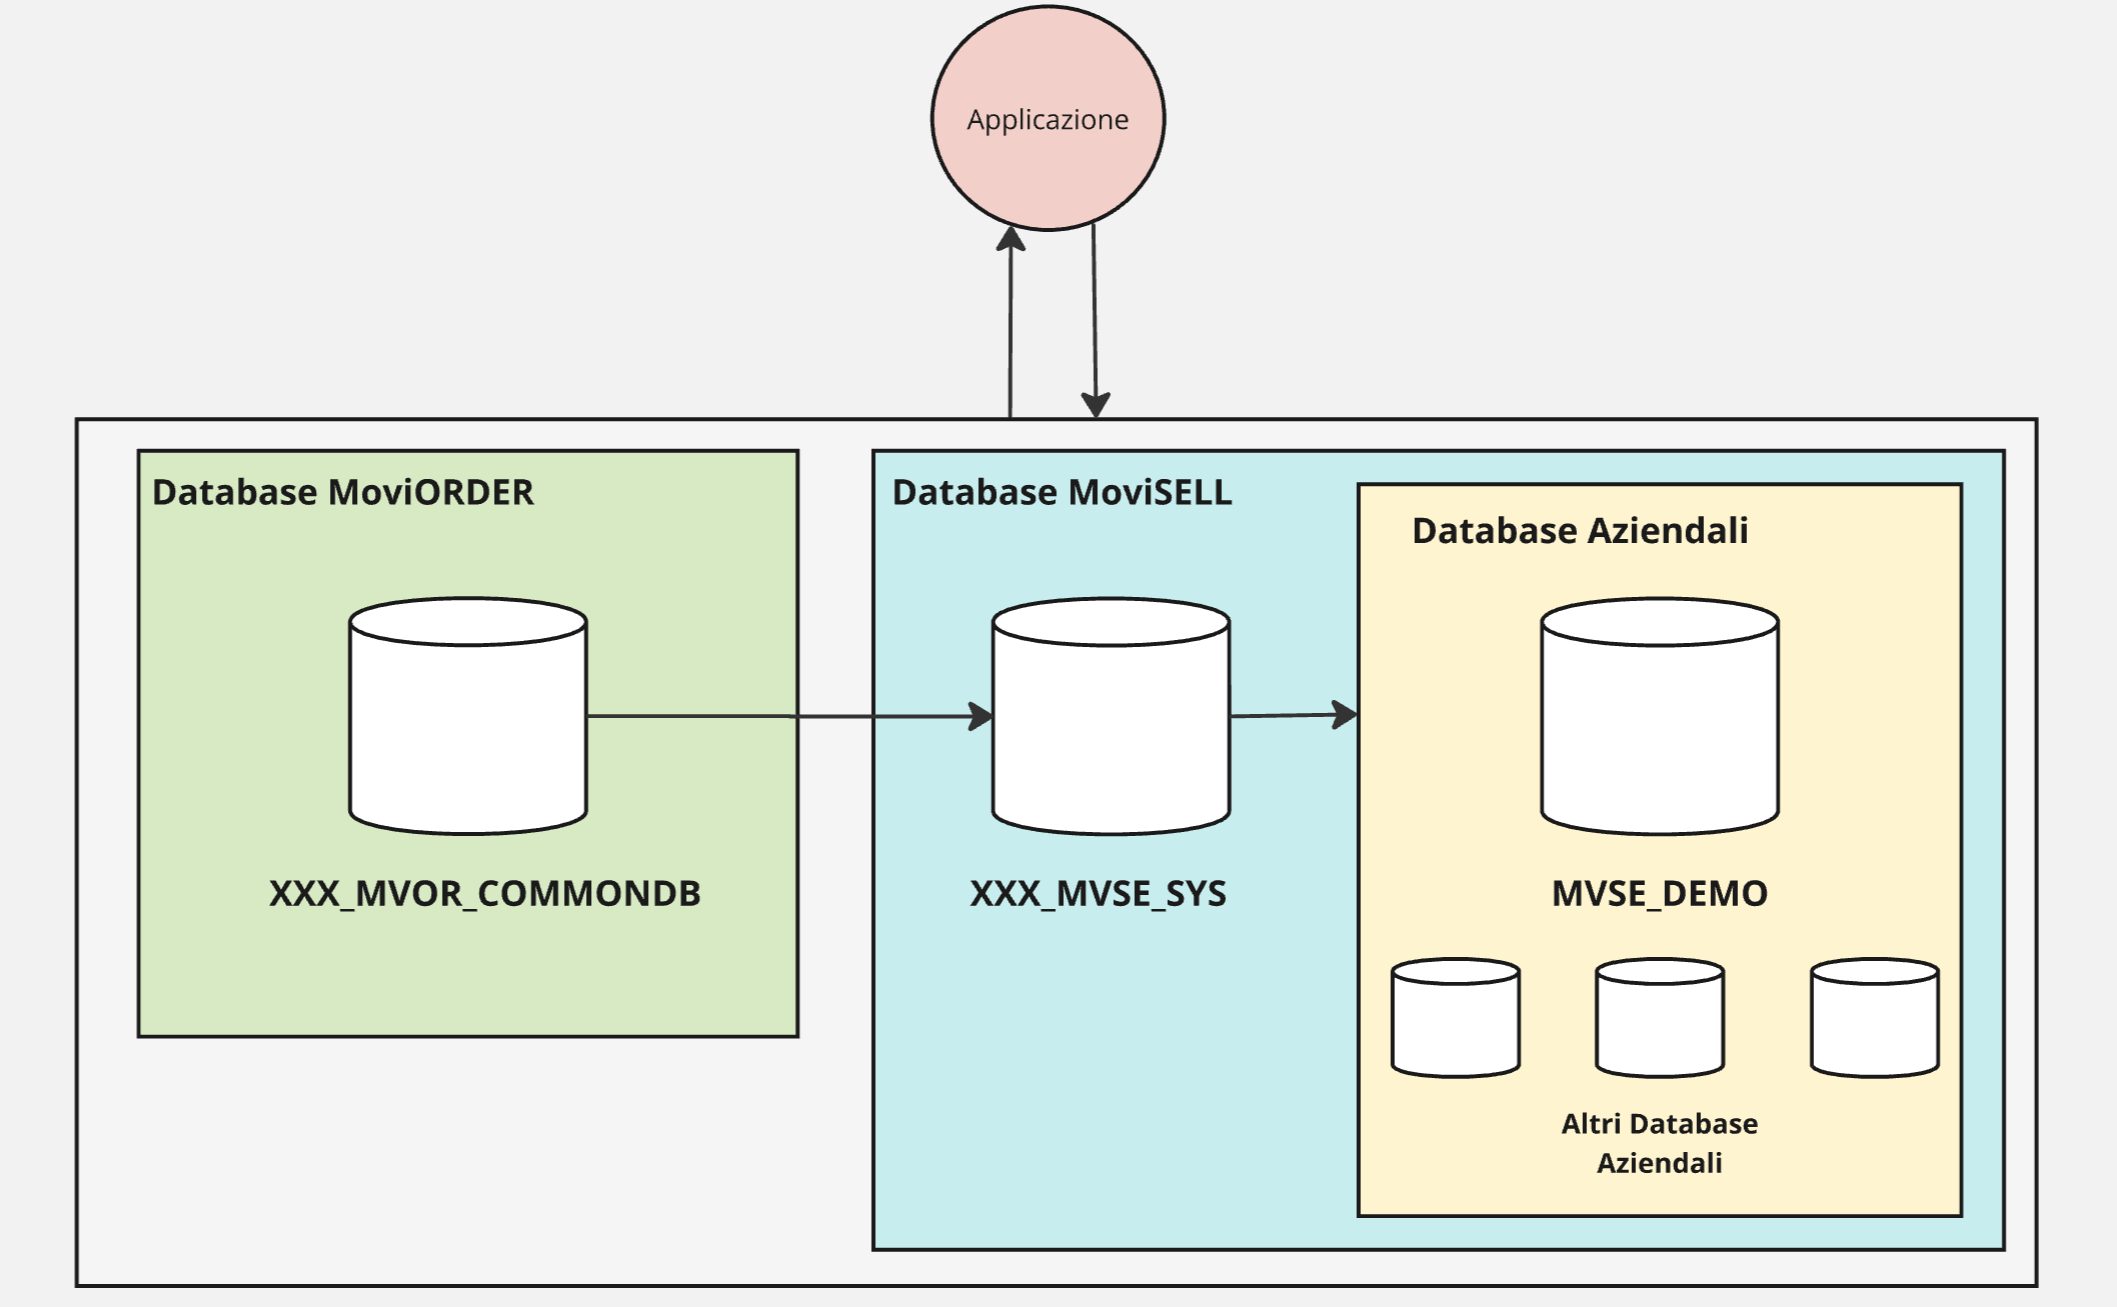
\includegraphics[alt={\textit{Database} di MoviORDER}, width=0.7\textwidth]{img/database.png}
    \caption {\textit{Database} di MoviORDER.}
    \label{fig:database}
\end{figure}

Come illustrato nella figura \ref{fig:database}, l'infrastruttura dati dell'applicazione {\movi} si articola su tre 
\textit{database} distinti: \textbf{XXX\_MVOR\_COMMONDB}, e i \textit{database} condivisi con l'applicazione 
MoviSELL, ovvero \textbf{XXX\_MVSE\_SYS} e \textbf{MVSE\_DEMO}.\\
XXX\_MVOR\_COMMONDB (che per brevità chiameremo \textit{common database}), contiene i dati relativi a gli utenti di MoviORDER. 
Esso conserva informazioni necessarie all'applicazione come: \textbf{credenziali di accesso, stato di validità della licenza, 
configurazioni dell'interfaccia utente, dettagli del dispositivo, indirizzi email} e altri parametri necessari al corretto 
funzionamento del \textit{software}. Questi dati sono fondamentali per i processi di autenticazione e inizializzazione 
dell'applicazione.\\
Ogni azienda ha il proprio \textit{database} dedicato, che chiameremo \textit{company}, in cui vengono conservati tutti i dati 
a lei inerenti come: \textbf{anagrafica clienti, catalogo prodotti, politiche di sconto personalizzate, profili degli agenti 
aziendali} ecc. Per ogni \textit{company database} viene assegnato un nome del tipo MVSE\_[nome azienda], nel mio caso per lavorare 
in locale mi è stato fornito un \textit{database} di prova chiamato MVSE\_DEMO.\\
Quindi abbiamo XXX\_MVSE\_SYS, il cui scopo è quello di fare da \textit{router}, infatti il \textit{common database} contiene un campo 
nella tabella \texttt{User} chiamato \texttt{CompanyCode} che agisce da chiave esterna assegnando ad ogni utente di {\movi} 
un \textit{database company} di riferimento. Questo \texttt{CompanyCode} viene utilizzato dalle \gls{api} come chiave per il 
\textit{router database} per ottenere la stringa di connessione al \textit{company database} durante la fase di autenticazione dell'
utente.\\
Questa architettura garantisce una gestione efficiente e scalabile dei dati, consentendo una separazione netta tra informazioni 
riguardanti l'applicazione e i dati specifici delle aziende, oltre a fornire un meccanismo flessibile per l'indirizzamento 
delle connessioni ai \textit{database} aziendali.

\subsection{Architettura delle API}
Ho continuato quindi il mio studio passando all'analisi dell'architettura delle \gls{api} che come accennato nel capitolo 
\ref{chap:vincoli tec} sono sviluppate utilizzando il \textit{framework} ASP.NET Core. 
Il \textit{back-end} di {\movi} si trova in una \textit{repository} BitBucket a sè stante rispetto al \textit{front-end} per consentire 
una gestione più efficiente e modulare del progetto. Questo permette: 
\begin{itemize}
    \item \textbf{Manutenibilità}: facilita la manutenzione e l'aggiornamento di ciascuna componente senza impattare l'altra;
    \item \textbf{Flessibilità tecnologica}: permette l'utilizzo di tecnologie e \textit{framework} diversi per \textit{back-end} e 
          \textit{front-end}, ottimizzando ciascuno per il proprio scopo e facilitando eventuali cambiamenti di tecnologie futuri;
    \item \textbf{Versionamento}: consente una versionamento separato per le due parti dell'applicazione e semplificando il 
          tracciamento delle modifiche del codice;
    \item \textbf{Riutilizzo del codice}: Facilita il riutilizzo del \textit{back-end} per diverse interfacce o applicazioni.
\end{itemize}

\begin{figure}[H]
    \centering
    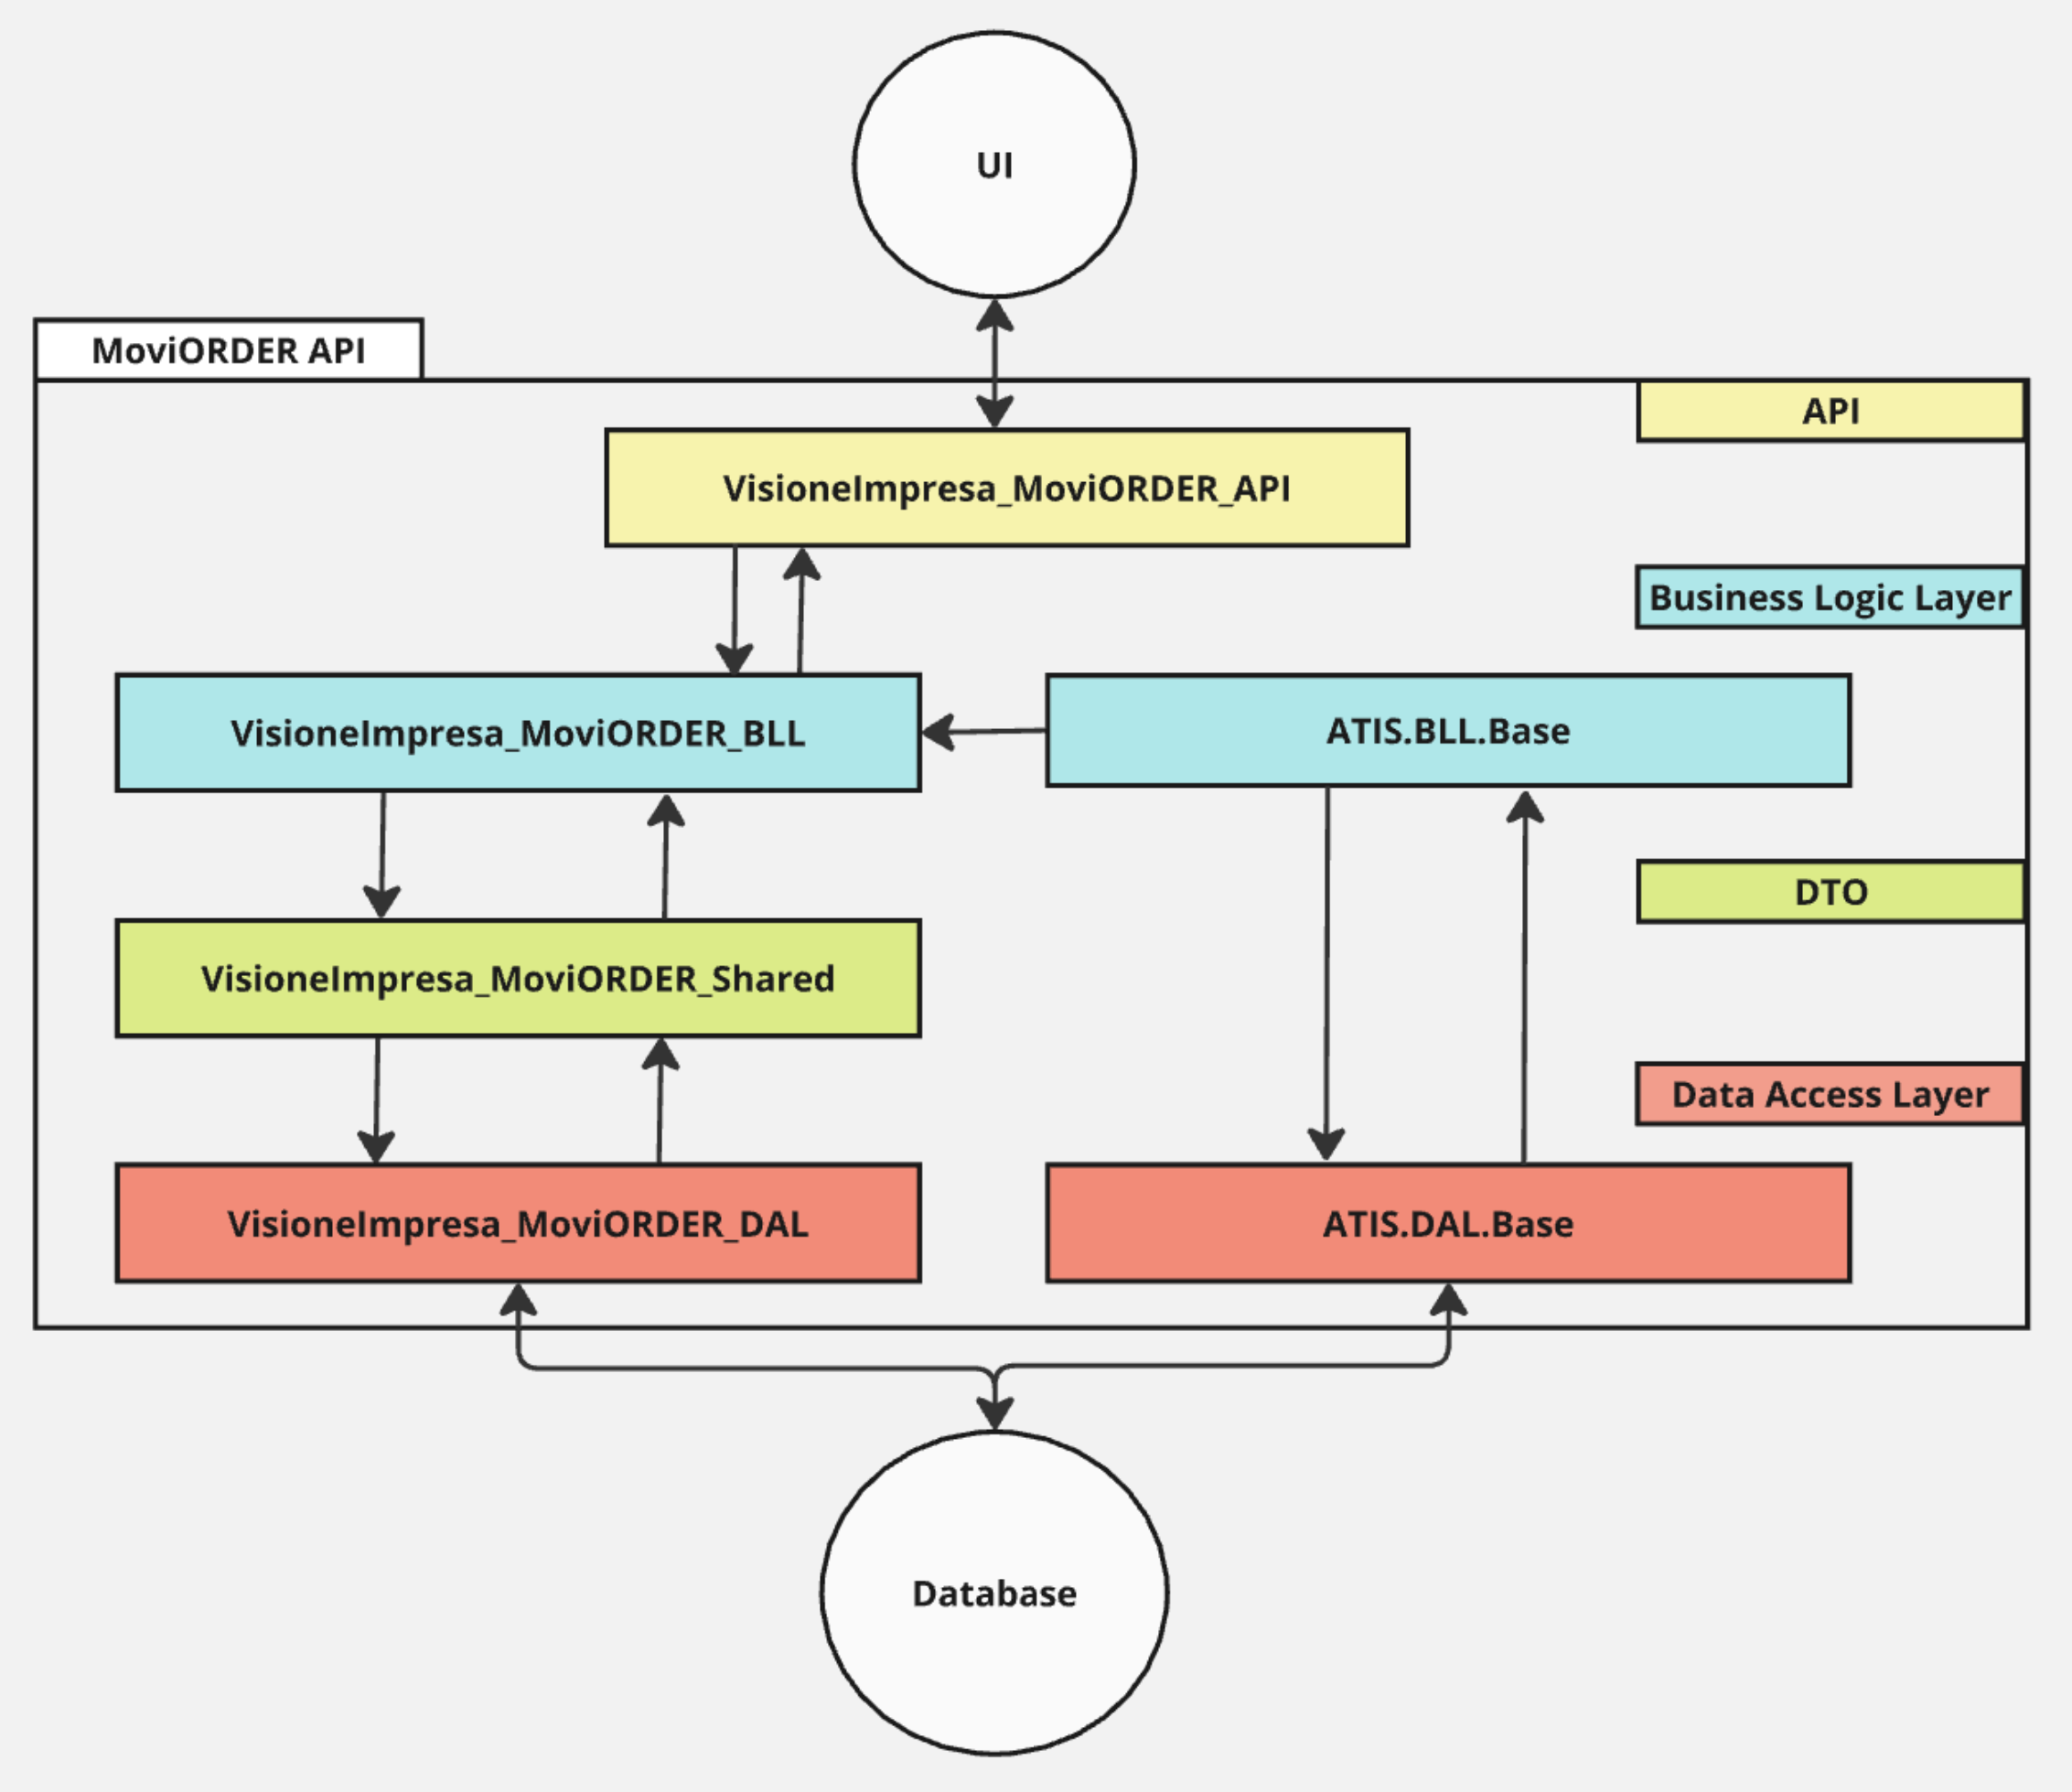
\includegraphics[alt={Architettura API}, width=0.7\textwidth]{img/multilayered.png}
    \caption {Architettura API.}
    \label{fig:multilayered}
\end{figure}

Le \gls{api} di {\movi} adottano un architettura di tipo \textit{layered}, come mostrato in 
figura \ref{fig:multilayered}. Questa architettura stratifica il codice in livelli di astrazione crescente, 
partendo dallo strato più "concreto" in diretta interazione con il \textit{database}, fino a quello più 
"astratto" che si interfaccia con il \textit{front-end}.
\subsubsection{Data Access Layer}
Partiamo analizzando la struttura dal livello più basso, ovvero il \textbf{\textit{Data Access Layer}}.\\
Alla base di questa architettura troviamo la cartella VisioneImpresa\_MoviORDER\_DAL che contiene i modelli e le \textit{migration} 
generate tramite Entity Framework, un \textit{mapper} ad alto livello integrabile a .NET che permette la  la trasposizione delle tabelle 
del \textit{database} in classi del dominio applicativo.\\
Entity Framework, originariamente parte del \textit{framework} .NET ma ora distribuito come pacchetto 
indipendente installabile attraverso l'\textit{installer} di Visual Studio, promuove un approccio di sviluppo 
\textit{code first}. Entity Framework permette infatti di gestire il \textit{database} attraverso i modelli, 
ovvero delle particolari classi che descrivono la forma della tabelle e i loro attributi.\\
Creando o modificando questi modelli è possibile creare o modificare la tabella della base dati senza senza la necessità di interventi 
manuali diretti, ma attraverso le \textit{migration} generate dal \textit{framework} automaticamente. 
Quando si apportano modifiche al modello, Entity Framework compara le \textit{migration} esistenti, determinando 
così lo stato attuale del \textit{database}. Questo processo permette di identificare precisamente le modifiche necessarie 
alla struttura del \textit{database}. Se il processo di analisi e generazione va a buon fine, Entity Framework crea una 
nuova \textit{migration} che riporta tutte le modifiche applicate. Questo meccanismo assicura una gestione coerente e 
tracciabile dell'evoluzione della struttura del \textit{database}, mantenendo sincronizzati il modello dei dati 
nell'applicazione e la struttura effettiva del \textit{database}.
\subsubsection{DTO Layer}
L'utilizzo diretto dei modelli come classi \textit{standard} presenta due criticità:
\begin{itemize}
    \item \textbf{Vulnerabilità nella sicurezza dei dati}: la creazione di istanze dirette dei modelli può esporre 
          involontariamente informazioni sensibili. Un esempio è la tabella \texttt{User} del \textit{common database}, 
          dove tra gli attributi troviamo la \texttt{password} dell'utente. L'utilizzo di queste 
          istanze potrebbe portare alla divulgazione accidentale di dati riservati in parti dell'applicazione dove 
          non sono necessari;
    \item \textbf{Limitazioni nella flessibilità strutturale}: i modelli generati rispecchiano fedelmente la struttura 
        del \textit{database}, ma spesso sono richieste rappresentazioni dei dati più sofisticate o personalizzate. 
          In molti casi, è preferibile definire classi che aggregano o rielaborano dati provenienti da più modelli, 
          offrendo una rappresentazione più adatta alle esigenze funzionali dell'applicazione.
\end{itemize}
Ecco perché viene introdotto un nuovo \textit{layer}, quello dei \textbf{DTO}.\\
All'interno della cartella VisioneImpresa\_MoviORDER\_Shared vengono definiti i DTO (\textit{Data Transfer Objects}), 
oggetti utilizzati per incapsulare e trasferire dati tra diversi componenti di un'applicazione.\\
Essenzialmente, sono contenitori di dati privi di logica di business, progettati per trasportare informazioni tra i 
componenti del sistema. I DTO tipicamente contengono solo proprietà pubbliche, senza implementare comportamenti complessi, 
permettendo di controllare precisamente quali dati vengono esposti e trasferiti, migliorando significativamente la 
sicurezza del sistema. 
Questo è particolarmente importante per proteggere informazioni sensibili, come \textit{password} o altri dati riservati, 
che possono essere omessi o mascherati.\\
L'utilizzo dei DTO incrementa anche la manutenibilità del codice, introducendo un livello di astrazione tra la 
struttura del \textit{database} e la logica applicativa. Questo disaccoppiamento facilita la manutenzione e 
l'evoluzione del codice, permettendo modifiche alla struttura del \textit{database} o alla \textit{business logic} 
senza impattare direttamente le interfacce esposte.
\subsubsection{Business Logic Layer}
Risalendo l'architettura, incontriamo il \textbf{\textit{Business Logic Layer}}, la cui implementazione è contenuta 
nella cartella VisioneImpresa\_MoviORDER\_BLL. In questo strato è definita la logica che governa il comportamento 
delle \gls{api}.\\
La struttura del \textit{Business Logic Layer} è organizzata in tre sottocartelle principali, ciascuna con un ruolo specifico:
\begin{itemize}
    \item \textbf{\textit{Mappings}}: questa sezione ospita i \textit{mapper}, componenti che facilitano la conversione 
          tra i modelli del \textit{database} e i DTO e viceversa. I \textit{mapper} garantiscono una corretta conversione 
          dei dati, preservando l'integrità delle informazioni mentre si muovono attraverso il sistema. Inoltre, definiscono 
          relazioni tra diversi DTO, permettendo una gestione profonda delle strutture dati all'interno del sistema;
    \item \textbf{\textit{Interfaces}}: qui sono definite le interfacce che descrivono i contratti per i metodi implementati 
          nei servizi. Queste interfacce permettono di promuovere un \textit{design} basato sui principi SOLID, 
          in particolare il principio di inversione delle dipendenze. L'inversione delle dipendenze stabilisce che i moduli 
          di alto livello non dovrebbero dipendere direttamente dai moduli di basso livello, ma entrambi dovrebbero dipendere 
          da astrazioni. Nel contesto di {\movi}, questo si traduce nel fatto che i componenti che utilizzano i servizi del 
          \textit{Business Logic Layer} (come i controller nell'\textit{API Layer}) dipendono dalle interfacce anziché 
          dalle implementazioni concrete dei servizi. L'uso di interfacce facilita il disaccoppiamento 
          tra i componenti, migliora la testabilità del codice e permette una maggiore flessibilità nell'implementazione e 
          nella manutenzione del sistema;
    \item \textbf{\textit{Services}}: questa cartella contiene le implementazioni concrete dei metodi definiti nelle interfacce. 
\end{itemize}
\subsubsection{Classi di supporto}
Come si vede nella figura \ref{fig:multilayered} sono presenti due \textit{directory} che non sono ancora state discusse: 
\textbf{ATIS.BLL.Base e ATIS.DAL.Base}. Qui sono contenute una serie di classi e implementazioni di metodi speciali 
per la gestione delle operazioni CRUD (\textit{Create Read Update Delete}) e per la gestione dell'architettura a più 
\textit{database} tramite classi come \texttt{DBContext} che permettono di selezionare e operare sul \textit{database} 
corretto. In ATIS.BLL.Base troviamo la definizione delle classi di supporto e la definizione del metodi, mentre in 
ATIS.DAL.Base 

                        TODO SCRIVERE E SISTEMARE, REPOSITORY PATTERN 

Nel contesto dello sviluppo \textit{software}, il pattern Repository è un'importante astrazione per la gestione delle operazioni di accesso ai dati. Le interfacce IReadOnlyRepository<TContext>, IRepository<TContext>, e IBaseService<TContext, TEntity> implementano questo pattern, fornendo un'architettura che separa la logica di accesso ai dati dalle operazioni di business. Queste interfacce permettono di gestire in modo efficiente le operazioni di lettura, scrittura, aggiornamento ed eliminazione delle entità all'interno di un contesto (TContext) che estende DbContext.

Interfaccia IReadOnlyRepository<TContext>
L'interfaccia IReadOnlyRepository<TContext> definisce operazioni di sola lettura sulle entità di un database. Tramite i metodi offerti, è possibile recuperare singole entità o insiemi di entità, basandosi su criteri di filtro opzionali. Ad esempio, il metodo GetQueryable<TEntity> restituisce un oggetto IQueryable<TEntity> che permette di costruire query personalizzate, mentre GetById consente di recuperare un'entità specifica tramite il suo identificatore. I metodi asincroni (GetByIdAsync, GetExistsAsync) sono essenziali per migliorare le prestazioni in contesti dove la reattività dell'applicazione è cruciale.

Interfaccia IRepository<TContext>
IRepository<TContext> estende IReadOnlyRepository<TContext> aggiungendo le operazioni di scrittura, aggiornamento ed eliminazione. Questa interfaccia completa le funzionalità CRUD (Create, Read, Update, Delete) necessarie per gestire il ciclo di vita delle entità in un'applicazione. I metodi Create e CreateAsync permettono di inserire nuove entità nel contesto, mentre Update e UpdateRange gestiscono la modifica delle entità esistenti. Per la rimozione delle entità, sono disponibili metodi come Delete e DeleteRange. Inoltre, Save e SaveAsync consentono di salvare le modifiche apportate al contesto nel database, garantendo la persistenza dei dati.

Interfaccia IBaseService<TContext, TEntity>
L'interfaccia IBaseService<TContext, TEntity> offre un livello di astrazione superiore, combinando operazioni di lettura e scrittura in un unico servizio generico. Questo servizio si integra con le interfacce di repository, fornendo un'interfaccia centralizzata per la gestione delle entità in un'applicazione. I metodi GetAllAsync, Get, Create, Update, e Delete coprono l'intera gamma di operazioni CRUD, mentre la gestione asincrona permette di ottimizzare l'interazione con il database in scenari ad alta concorrenza.

Utilizzo nel Contesto di un'Applicazione
In un'applicazione tipica, queste interfacce vengono implementate da classi concrete che interagiscono direttamente con il database. IReadOnlyRepository potrebbe essere utilizzato in contesti dove le operazioni di lettura sono prevalenti, come nei servizi di reportistica. IRepository viene invece utilizzato in servizi che richiedono operazioni complete di manipolazione dei dati. IBaseService offre un'interfaccia di servizio che incapsula le operazioni di repository, promuovendo la riusabilità e la manutenibilità del codice.

Queste interfacce, utilizzate insieme, permettono di strutturare in modo efficace l'accesso ai dati, mantenendo separata la logica di business dalla logica di persistenza, e favorendo la scrittura di codice più modulare, testabile e manutenibile.


\subsubsection{API Layer}
Il \textit{layer} più alto nell'architettura è l'\textit{\textbf{API Layer}}, implementato nella cartella 
VisioneImpresa\_MoviORDER\_API.\\
Questo strato rappresenta il punto di contatto tra il sistema \textit{back-end} e il \textit{front-end}, 
le \gls{api} definite in questo layer agiscono come punti di ingresso per le richieste esterne: ogni \gls{api} espone 
una firma e richiede i dati in un formato predefinito.\\
All'interno della definizione di ciascuna \gls{api}, viene invocato il corrispondente metodo definito nel livello sottostante.\\
I risultati vengono quindi restituiti all'interfaccia utente.\\
In questo livello troviamo inoltre:
\begin{itemize}
    \item \textbf{\texttt{Program.cs}}: questo file è il punto di ingresso dell'applicazione, dove viene configurato e avviato il 
           server web che ospita le \gls{api};
    \item \textbf{Configurazione di Swagger}: ovvero lo strumento usato per il \textit{testing} delle \gls{api};
    \item \textbf{Definizione degli \textit{endpoint}}: ovvero gli indirizzi di connessione ai vari \textit{database} 
          e l'indirizzo in cui le \gls{api} vengono esposte.
\end{itemize}
\subsection{Architettura Front-end}
                                          TODO SCRIVERE MEGLIO E GRAFICO
Infine ho studiato l'architettura del \textit{front-end}.\\
{\movi} come la maggior parte delle applicazioni React è strutturata secondo un'architettura chiamata \textit{component 
based}, che favorisce la modularità e il riutilizzo del codice.\\
Per componente in questo contesto intendiamo un gruppo di funzionalità correlate che risiede dietro un'interfaccia ben definita.
L'organizzazione del codice in questa architettura viene strutturato dividendo le varie parti per aree tematiche, 
migliorando la manutenibilità e la scalabilità del progetto.\\
La \textit{repository} è suddivisa nelle seguenti cartelle:
\begin{itemize}
    \item \textbf{Android}: specifica per React Native, contiene i file di configurazione 
          per la versione Android dell'\textit{app} e \textit{file} come \texttt{build.gradle} e \texttt{AndroidManifest.xml} 
          per la configurazione del compilatore Android;
    \item \textbf{iOS}: specifica per React Native, contiene il progetto Xcode e i file di configurazione 
          per la versione iOS dell'\textit{app} e \textit{file} per la configurazione del compilatore di iOS;
    \item \textbf{lang}: contiene i \textit{file} \texttt{en.json e it.json} che contiene il testo usato nell'applicazione 
          in italiano e inglese;
    \item \textbf{src}: contiene tutto il codice del \textit{front-end} e realizza l'architettura \textit{component 
          based} che sarà descritta in seguito;
    \item \textbf{\textit{file} di varia natura nella root della \textit{repository}}: questi \textit{file} sono fondamentali 
          per garantire un corretto funzionamento e una gestione efficiente del progetto, qui riporto quelli più importanti:
          \begin{itemize}
            \item \textbf{\texttt{package.json}}: contiene le informazioni sul progetto come \textbf{nome del progetto, versione,
                  script di comando e dipendenze}. È il file principale per gestire i pacchetti Node.js utilizzati nel progetto;
            \item \textbf{\texttt{yarn.lock}}: questo file viene generato automaticamente quando si genera il progetto e 
                  permette di gestire ed installare le dipendenze del progetto con le loro versioni esatte;
            \item \textbf{\texttt{metro.config.js}}: configurazione di Metro, il \textit{bundler} di JavaScript predefinito 
                  per React Native. Questo file permette di personalizzare il comportamento di Metro, come 
                  l'aggiunta di alias, path customizzati, o l'esclusione di determinati file dalla build.
            \item \textbf{\texttt{babel.config.js}} babel.config.js: Configura Babel, il transpiler di JavaScript. 
                  Definisce come il codice deve essere trasformato per essere compatibile con le varie versioni di JavaScript e i 
                  diversi ambienti in cui verrà eseguito.
            \item \textbf{\texttt{index.js}} index.js: Punto d'ingresso principale dell'applicazione React Native. Qui viene 
                  avviato il rendering del componente radice dell'\textit{app}, generalmente importando e registrando il componente 
                  principale.
            \item app.tsx: Contiene il componente radice dell'applicazione. Qui vengono definiti l'interfaccia utente principale 
                  e la logica di base dell'\textit{app}.
            \item tsconfig.json: Configura il compilatore TypeScript, specificando le opzioni di compilazione e il comportamento del transpiling del codice TypeScript in JavaScript.
          \end{itemize}
\end{itemize}

Descriviamo ora ogni area della cartella src,
\begin{itemize}
      \item Cartella components": Contiene componenti riutilizzabili e generici, suddivisi ulteriormente in sottocartelle come "ui" per elementi dell'interfaccia utente e "layout" per strutture di pagina comuni.
      \item Cartella "pages" o "views": Ospita componenti che rappresentano intere pagine o viste principali dell'applicazione.
      \item Cartella "services": Contiene moduli per la gestione delle chiamate API e la logica di business condivisa.
      \item Cartella "hooks": Raccoglie hook personalizzati per la gestione dello stato e della logica riutilizzabile.
      \item Cartella "context" o "store": Dedicata alla gestione dello stato globale dell'applicazione, sia utilizzando il Context API di React che soluzioni come Redux.
      \item Cartella "utils" o "helpers": Per funzioni di utilità e helper condivisi in tutta l'applicazione.
      \item Cartella "assets": Per risorse statiche come immagini, font e file di stile globali.
\end{itemize}
Questa organizzazione per aree facilita la navigazione nel codice e promuove una chiara separazione delle responsabilità. 
React utilizza un flusso di dati unidirezionale, dove le informazioni fluiscono dall'alto verso il basso attraverso le 
proprietà (props), mentre lo stato dell'applicazione è gestito attraverso soluzioni di gestione dello stato.
